
\section{Algoritmos de predicción} % (fold)
\label{sec:algoritmos_de_prediccion}

\subsection{Regresión Logística} % (fold)
\label{sub:regresion_logistica}

La regresión logística a pesar de su nombre es un algoritmo de clasificación, el cual puede implementarse para realizar una clasificación binaria, o una clasificación de múltiples valores posibles.

El modelo de la regresión logística es análogo al de la regresión lineal, dado que tal como la misma, parte de una función hipótesis que se le aplica a los datos de entrada.
\begin{equation}
h_{\theta}(x)= \theta^T \cdot x
\end{equation}
\begin{small}
Esta es la representación vectorial de la función hipótesis de la regresión lineal. Donde $X$ es el vector traspuesto de datos $x_{i}$, y $\Theta^T$ es el vector de pesos $\theta_{j}$.
\end{small} \newline

En el caso de la regresión lineal, el valor de retorno de la función hipótesis puede variar mucho dependiendo del vector de datos de entrada $X$ y el vector de pesos $\Theta$. En este aspecto la regresión logística se diferencia de la regresión lineal.

\subsubsection{Función sigmoidal.}
En el caso particular de la regresión logística, la función hipótesis se construye de la siguiente manera:
\begin{equation}
h_{\theta}(x)= \frac{1}{1+e^{- \theta^T\cdot x }}
\end{equation}

Similarmente, la hipótesis de la regresión logística utiliza el vector de datos de entrada $X$ y el de pesos $\Theta$, y su función retorna un valor escalar. Sin embargo, esta nueva función otorga una ventaja al retornar un número escalar real comprendido entre 1 y 0. Este tipo de función se llama función sigmoidal, y el valor escalar comprendido entre 1 y 0 se puede interpretar como una probabilidad.
\begin{figure}[H]
\centering
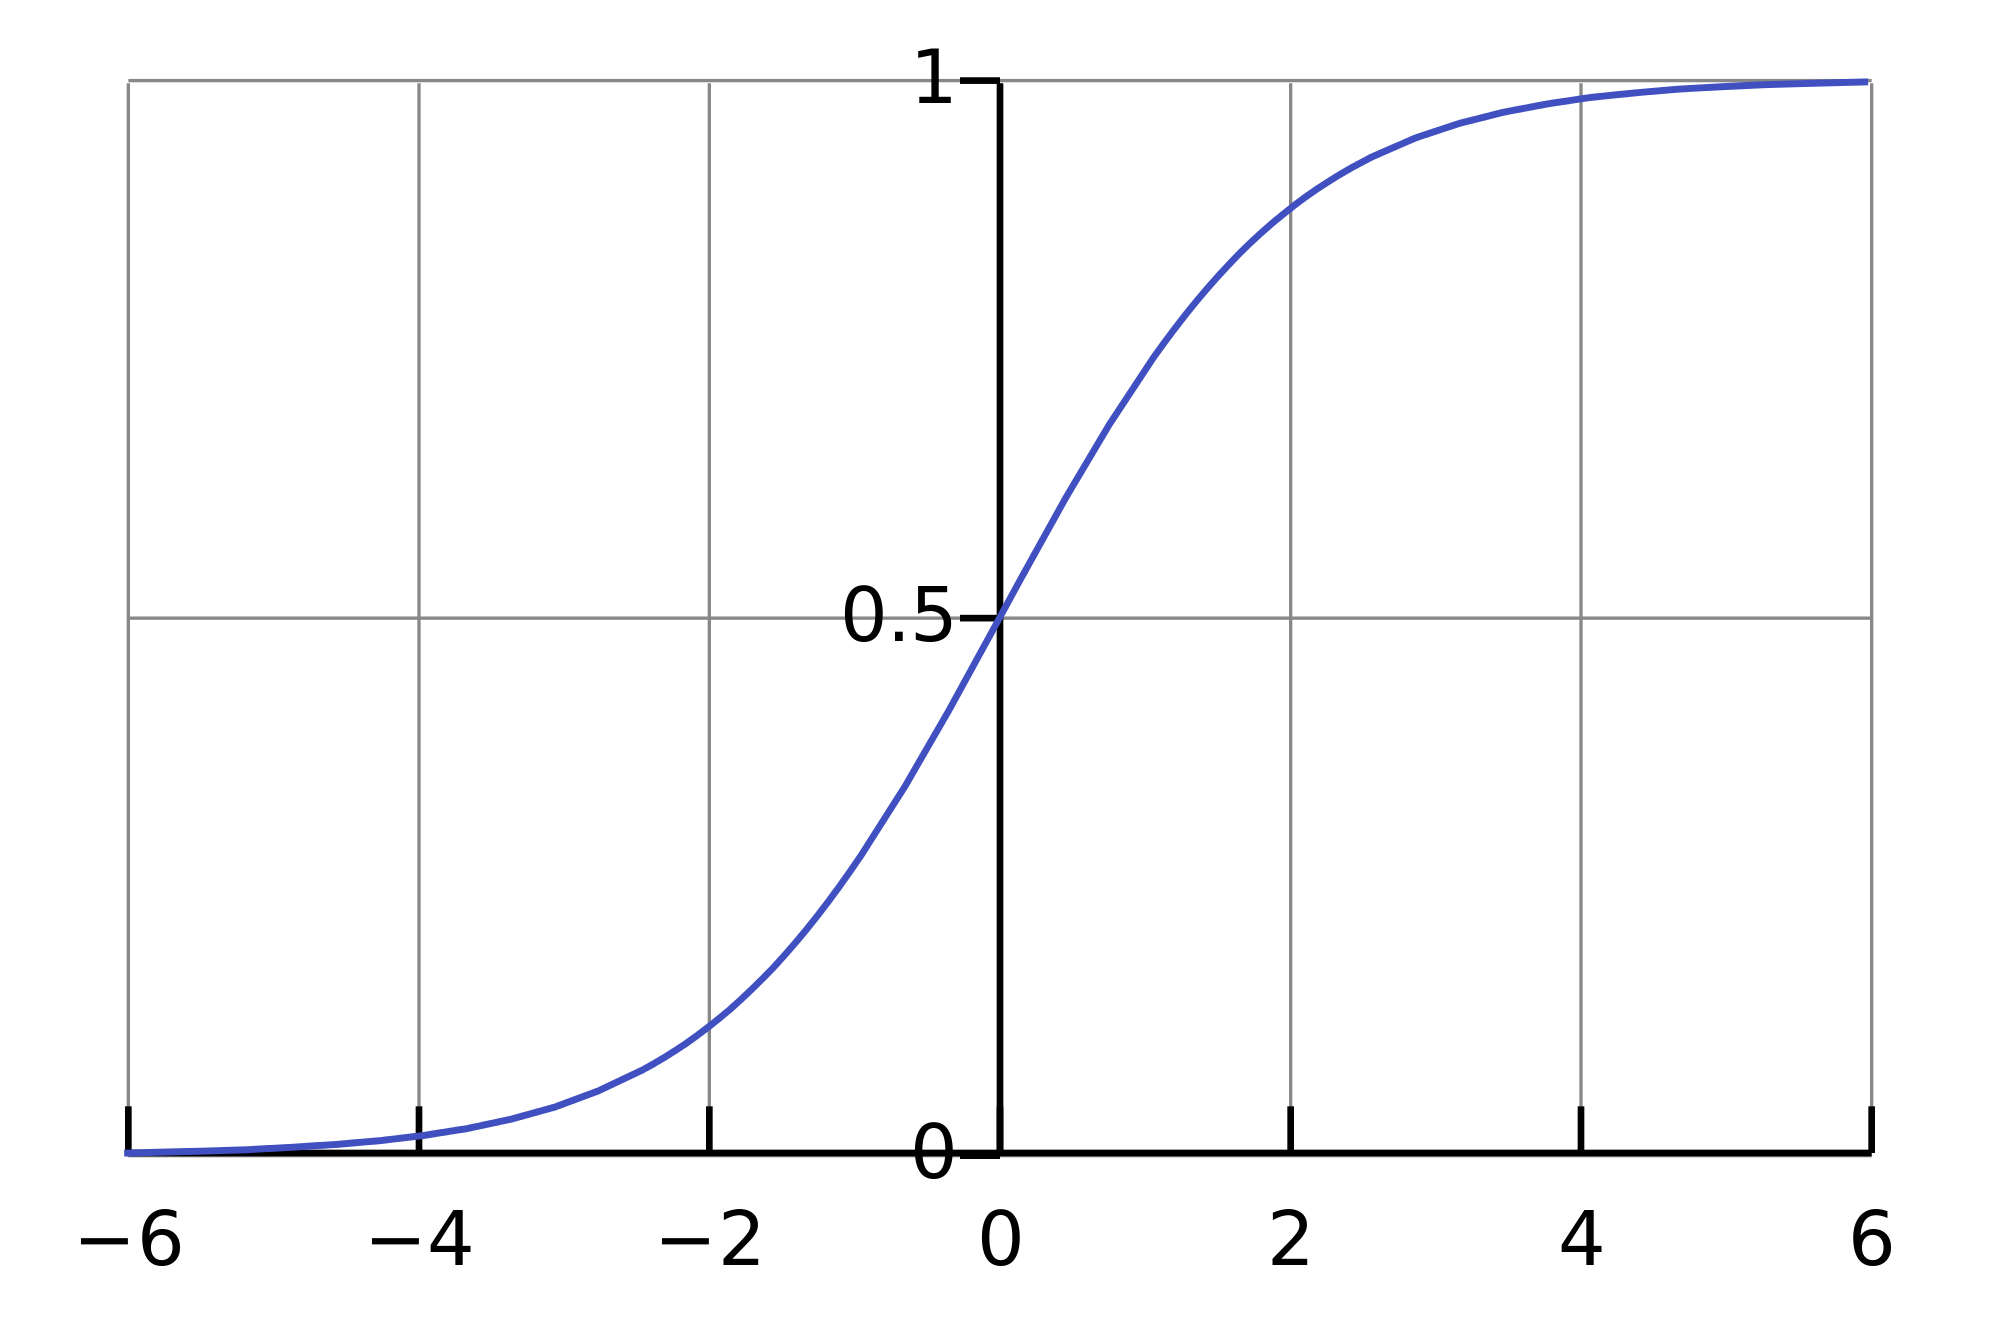
\includegraphics[width=80mm]{logisticCurve}
\caption{Gráfica de una función sigmoidal.}
\label{fig:logisticCurve}
\end{figure}

\subsubsection{Uno contra todos.}
Sin embargo, hasta el momento el algoritmo parece ser sólo diseñado para resolver problemas de clasificación binaria. Para utilizar este algoritmo de forma pueda abordar un problema de salida multiclase, debe aplicarse algún esquema de clasificación que aproveche las salidas binarias (o de probabilidad entre 0 y 1) de la función sigmoidal. Para eso se utiliza el esquema \textit{ovr (One-vs-rest)}. One-vs-rest no aplica otra cosa que el criterio de \textit{dividir y conquistar}. Por cada clase se resuelve el problema en forma binaria, donde el caso positivo (1) corresponde a la clase misma, y el caso negativo corresponde a cualquier otra clase. A continuación puede verse una representación gráfica de esta estrategia:

\begin{figure}[H]
\centering
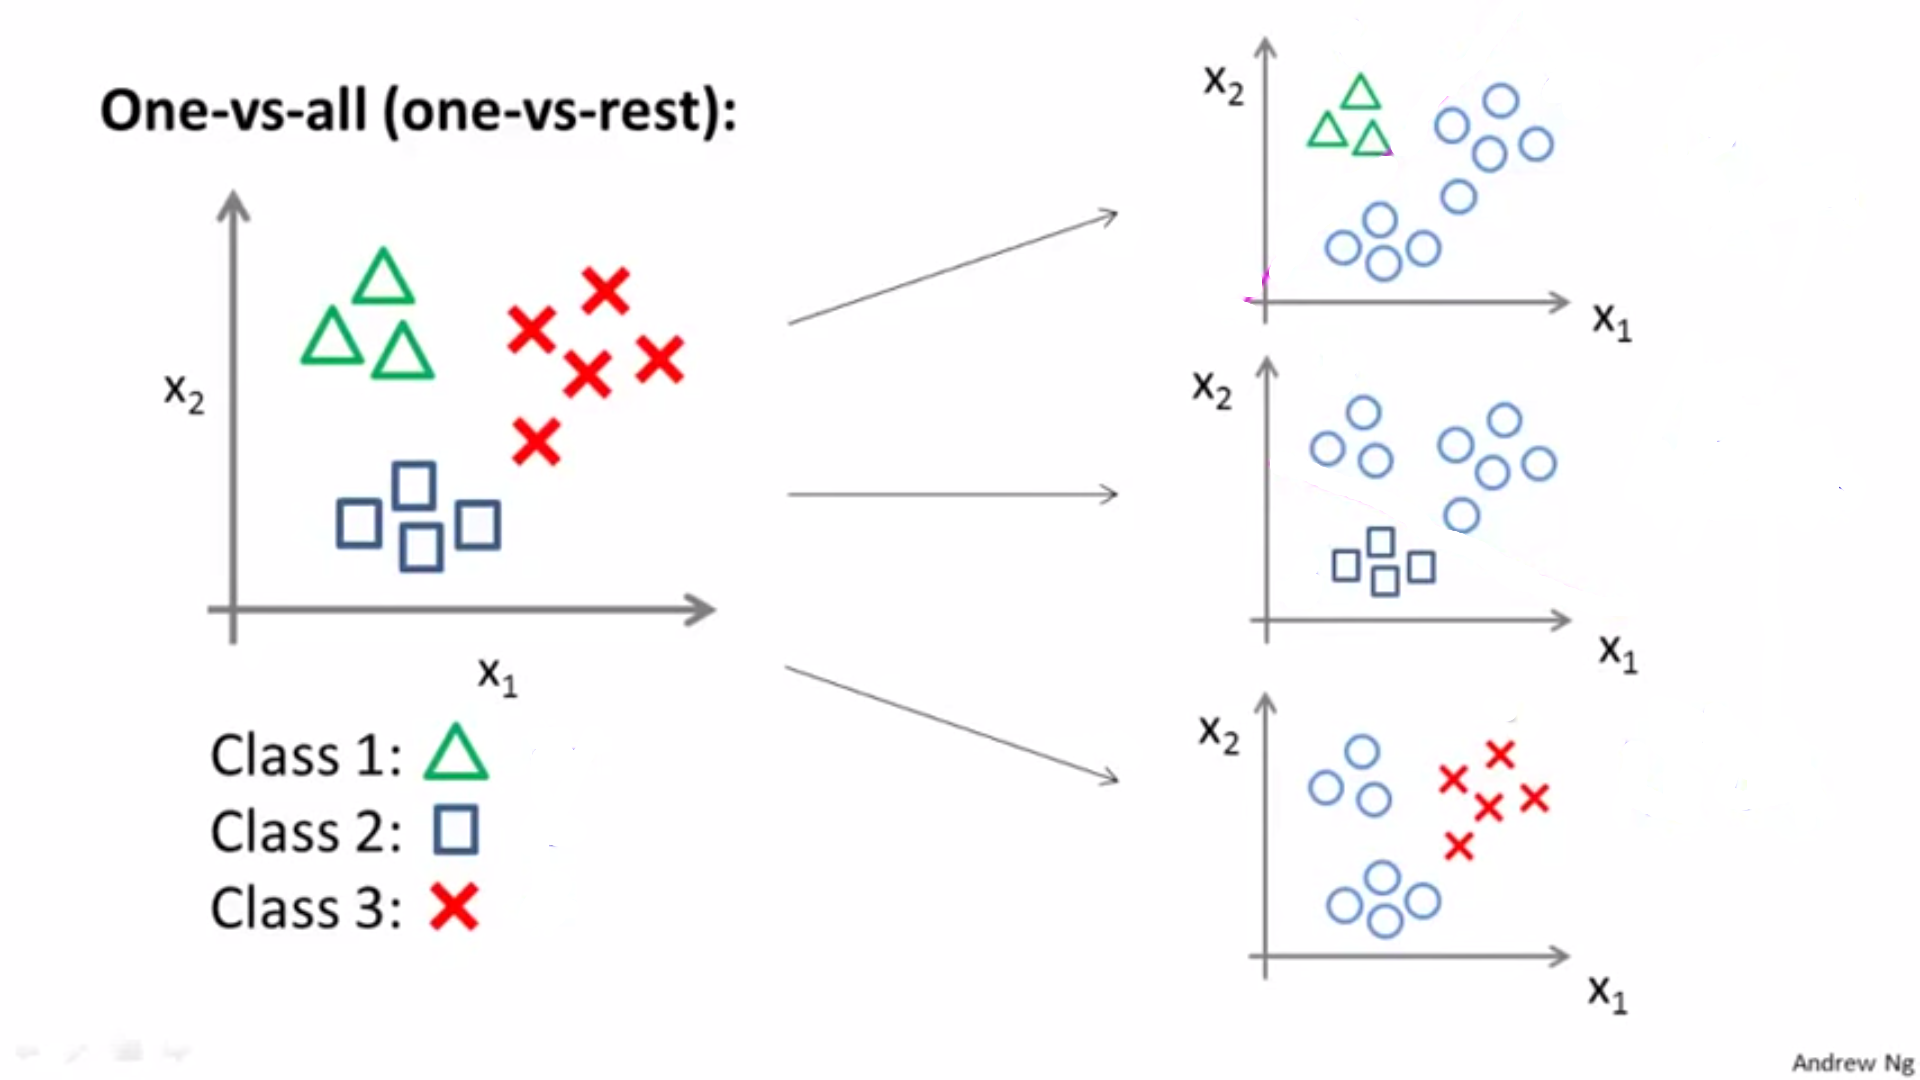
\includegraphics[width=80mm]{oneVsRest}
\caption{Representación gráfica one-vs-rest. \cite{AndrewNgMulticlass}}
\label{fig:oneVsRest}
\end{figure}

\subsubsection{Estimación y Función de Costo.}
De esta manera se cuenta con una serie de funciones $h_{\theta}^k(x)$ donde $k$ es el número de la clase que representa la función. A través del valor de retorno de todas estas funciones se obtiene entonces la probabilidad de cada clase distinta para cada caso del set de valores de entrada.

Este conjunto de probabilidades obtenido, es una estimación, y esa estimación debe aproximarse al valor deseado. En este trabajo disponemos de un set de entrenamiento asociado a las clasificaciones correctas. El objetivo de la regresión logística es esbozar una función de costo dados los pesos $\theta_{j}$ . De esta manera, optimizando (o minimizando) la función costo se pueden corregir los pesos $\theta_{j}$, de forma que las estimaciones posteriores se asemejen cada vez más a los valores deseados o ``correctos''.

A continuación se muestra un ejemplo ilustrativo de una definición de función de costo:

\begin{equation}
J(h_{\theta }(x),y) = \begin{cases}
- \log h_{\theta}(x) & \textit{si $y \equiv 1$} \\
- \log (1- h_{\theta}(x)) & \textit{si $y \equiv 0$}
\end{cases}
\end{equation}

La conveniencia de esta función de costo es que:

\begin{itemize}
  \item Cuando el valor esperado es $1$, y la estimación se aproxima a $0$, el costo tiende a $\infty$.
  \item Cuando el valor esperado es $1$, y la estimación se aproxima a $1$, el costo tiende a $0$.
  \item Cuando el valor esperado es $0$, y la estimación se aproxima a $1$, el costo tiende a $\infty$.
  \item Cuando el valor esperado es $0$, y la estimación se aproxima a $0$, el costo tiende a $0$.
\end{itemize}

Esto ocurre gracias a que las funciones logarítmicas de cada caso se comportan como describen las siguientes gráficas:

\begin{figure}[H]
\centering
\begin{subfigure}{.5\textwidth}
  \centering
  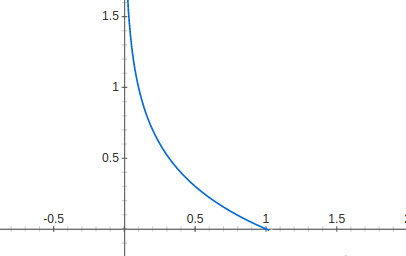
\includegraphics[width=.8\linewidth]{minusLogX}
  \caption{$y = - \log (x)$}
  \label{fig:minusLogX}
\end{subfigure}%
\begin{subfigure}{.34\textwidth}
  \centering
  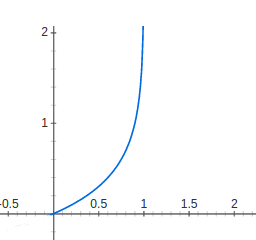
\includegraphics[width=.8\linewidth]{minusLog1minusX}
  \caption{$y = - \log (1-x)$}
  \label{fig:minusLog1minusX}
\end{subfigure}
\caption{Gráficas}
\label{fig:minusLog}
\end{figure}

Análogamente, se pueden definir funciones de costo de forma contínua, obteniendo comportamientos similares. En el caso particular de la clase LogisticRegression implementada en el paquete de python \textit{sklearn}, una función de costo utilizada es la siguiente:

\begin{equation}
J(\theta,c)= \theta^T \cdot \theta + C \sum_{i=1}^n \log (e^{-y_{i} \cdot (X_{i}^T \theta + c)})
\end{equation}
Donde:

\begin{itemize}
  \item $X_{i}$ es el vector de parámetros de entrada del i-ésimo caso de un set de entrenamiento.
  \item $y_{i}$ es el valor correcto conocido del i-ésimo caso de un set de entrenamiento.
  \item $c$ es una constante de ajuste, al igual que los pesos comprendidos en el vector $\theta$.
  \item $\theta^T \cdot \theta$ y $C$ son complementos de la función de costo pensados para regularizarla, suavizando su comportamiento con el fin de evitar cometer \textit{overfitting}.
\end{itemize}

\subsubsection{Optimización: descenso por el gradiente.}
Por último, queda detallar el método de optimización utilizado por la regresión logística. Los métodos de optimización de la función de costo pueden ser derivativos o no derivativos.

El método derivativo clásico es el descenso por el gradiente. El descenso por el gradiente consiste en calcular el gradiente de la función costo. De esta forma se obtiene la dirección y sentido de máximo crecimiento de la función. Con el fin de minimizarla, lo que se hace es, a través de un escalar que se denomina \textit{paso} de la optimización, se van variando los valores de $\theta_{i}$ en la misma dirección y sentido opuesto que el gradiente, de forma de apuntar hacia la minimización de la función de costo. Esto se realiza iterativamente, recalculando el gradiente de la función costo con los parámetros $\theta_{i}$ actualizados.

Sin embargo, las librería \textit{sklearn} utiliza en el modo \textit{liblinear} un método no derivativo denominado \textit{descenso coordenado} \cite{sklearnLinearModel}. El descenso coordenado consiste en partir la optimización en optimizaciones más simples, de una variable. Esto lo hace minimizando la función de costo por una coordenada o variable a la vez. Itera por cada variable y calcula la dirección de descenso de la función modificando el valor de esa sola variable.

A continuación se muestra una gráfica que ilustra este método de optimización:

\begin{figure}[H]
\centering
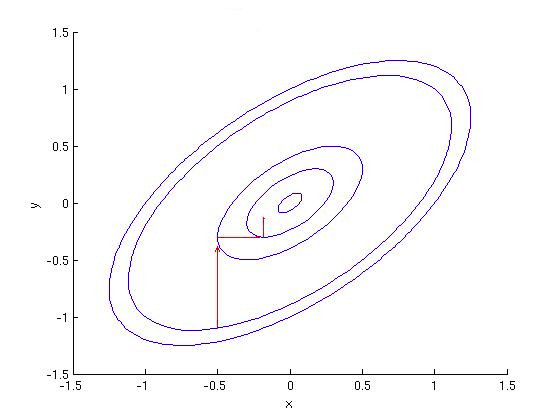
\includegraphics[width=80mm]{coordinateDescent}
\caption{Descenso coordenado. Las elipses concéntricas son curvas de nivel, donde el centro de las elipses se encuentra un mínimo local. \cite{wikipediaCoordinateDescent}}
\label{fig:coordinateDescent}
\end{figure}

En su forma vectorial, el descenso por el gradiente podría verse con la siguiente fórmula de actualización:
\begin{equation} \label{eq:gdesc}
\theta := \theta - \alpha \nabla J(\theta)
\end{equation}

\subsubsection{Feature Scaling}
Una mejora muy grande que se le puede hacer al descenso por el gradiente es la normalización o escalado de las variables de entrada (features). El problema que ataca es la diferencia entre los rangos de valores posibles de las features. 

Por ejemplo, una variable puede ser la cantidad de cuartos que tiene una casa y otro la cantidad de metros cuadrados que tiene. Mientras uno se mueve entre 1 y 10 aproximadamente, el otro seguro será 10 veces más grande. Otros más comunes son, por ejemplo, la calificación del 1 al 5 de una película contra la cantidad de vistas que tiene, que pueden ser millones. Este desequilibrio produce, en gráficos como la figura \ref{fig:coordinateDescent}, que se haga cada vez más ovalado, y por lo tanto el paso $\alpha$ que tiene que dar en cada iteración para que no haya divergencia tiene que ser menor. Esto hace que sea más difícil de debuggear y que la convergencia, debido al paso más chico, sea mucho más lenta.

El feature scaling consiste en pasar todas las variables a intervalos aproximadamente entre 0 y 1 y luego entrenar $\theta$ sobre esas nuevas features normalizadas. El scaling se hace de la siguiente manera:

\begin{equation}
x_i := \frac{x_i - \mu_{x_i}}{\sigma_{x_i}}
\end{equation}

Al quitarle el valor medio y dividir por la desviación estandar, todas las variables quedan en rangos similares y el descenso por el gradiente puede hacerse de forma más segura y rápida.

Para poner un ejemplo concreto, probando un ajuste de parábolas por regresión lineal, sin escalamiento de variables requería un $\alpha$ más pequeño que 0.0001 para converger y por lo tanto miles de iteraciones. Por otro lado, escalando las variables, había convergencia con un paso de 1.0 y en algunas decenas de iteraciones ya se conseguían errores menores a $10^{-15}$.

\subsubsection{Regularización}
Como fue mencionada antes, la regularización es una medida que se toma en contra del overfitting. El overfitting, o sobreajuste, es un problema que consiste en que el algoritmo predictor quede muy bien entrenado para el predecir dentro del set de entrenamiento, pero no tenga capacidad de generalizar. Esto suele ocurrir cuando se modela un problema con una complejidad mayor a la que le corresponde, o cuando faltan ejemplos para la cantidad de features que se proponen.

A veces quitar features no es una opción. Sin embargo, si se puede penalizar darle mucha importancia a todos los features a la vez. Esta penalización se hace a través del costo y se llama regularización:

\begin{equation}
J(\theta) = -\frac{1}{m}\sum_{i = 1}^{m}\left[y^{(i)}(log(h_\theta(x^{(i)}))) + (1-y^{(i)})log(1-h_\theta(x^{(i)}))\right] + \frac{1}{m}\sum_{j = 1}^{n}\theta_j^2
\end{equation}
Y en forma vectorial:
\begin{equation}
J(\theta) = \frac{1}{m}\left[ -y^Tlog(h_\theta(x)) - (1-y)^Tlog(1-h_\theta(x)) + \theta^T\theta\right]
\end{equation}

De todos modos hay que tener en cuenta que no se regulariza el parámetro del término independiente, con lo cual en el término de la derecha ($\theta^t\theta$) deben extraerse primero los $\theta_0$.

\subsubsection{Stochastic Gradient Descent}
Para conjuntos de datos muy grandes, tales como el que se nos presenta de crímenes en San Francisco, puede ser muy costoso sumar sobre todos los 800.000 ejemplos antes de avanzar un paso. El descenso por el gradiente estocástico, mezcla aleatoriamente los ejemplos y luego va iterando sobre aquellos, en cada paso bajando por la contribución que tiene cada uno al gradiente.

El descenso por el gradiente clásico (en tanda), según lo expuesto en la ecuación \ref{eq:gdesc}, puede expresarse componente a componente:
\begin{equation}
\theta_j := \theta_j - \alpha\frac{1}{m}\sum_{i = 1}^{m}(h_\theta(x^{(i)}) - y^{(i)})x_j^{(i)}
\end{equation}
Pero podemos observar que las componentes de la sumatoria son la parte que cada ejemplo contribuye al gradiente. Tomando este concepto, en lugar de sumar todos los valores antes de avanzar, el descenso por el gradiente estocástico baja un poco por cada ejemplo que recorre, a través de la contribución que este otorga al gradiente \cite{andrewStock}.

\begin{equation}
\theta_j := \theta_j - \alpha(h_\theta(x^{(i)}-y^{(i)}))x_j^{(i)}
\end{equation}
Esto último se hace para cada uno de los ejemplos y luego se vuelve a comenzar con el primero, hasta que el resultado sea el deseado.

Una variante de este método es una mezcla entre el descenso por el gradiente en tanda y estocástico, que agarra pequeñas tandas, de por ejemplo, 10 casos de entrenamiento cada una. Esto permite aprovechar las ventajas de vectorizar las cuentas que provee la versión en tanda y la ventaja de no tardar tanto tiempo hasta hacer un paso que provee la implementación estocástica.

\subsection{Redes Neuronales}
